\section{MLOps}

\begin{figure}[ht]
  \vspace{\baselineskip}
  \centering
  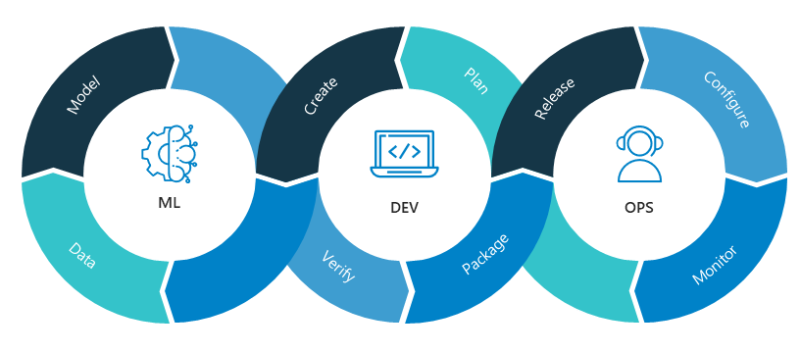
\includegraphics[width=0.8\textwidth]{02-mlops.png}
  \caption{Siklus hidup MLOps (Sumber:~\cite{mlops})}\label{fig:02-mlops-lifecycle}
\end{figure}

\subsection{Definisi MLOps}

MLOps adalah penerapan yang lebih spesifik dari DevOps. 
Seperti yang telah dibahas pada bagian sebelumnya, DevOps adalah suatu metodologi dan prinsip yang diterapkan untuk membuat proses pengembangan sistem menjadi lebih cepat dan efisien.
MLOps adalah metodologi yang menerapkan DevOps untuk proses-proses yang ada pada pengembangan model machine learning.
Gambar~\ref{fig:02-mlops-lifecycle} menunjukkan siklus dari MLOps secara umum.

Dalam MLOps, terdapat proses-proses tertentu yang spesifik untuk domain pengembangan sistem pemelajaran mesin (\cite{mlops}).\@
MLOps ini merupakan bidang yang masih baru karena baru-baru ini teknologi kecerdasan buatan mulai diterapkan dalam perusahaan yang mulai merambah ke layanan dengan kecerdasan buatan.
Tujuan dari MLOps adalah untuk melakukan manajemen dari eksperimen dalam proses pengembangan sistem pemelajaran mesin.
Saat ini, metodologi MLOps juga sudah diterapkan pada berbagai perusahaan besar di dunia, seperti Facebook, Google, AirBnB, dan Uber.

\subsection{Alasan MLOps Diperlukan}

Hal ini patut menjadi pertanyaan, ``apakah MLOps benar-benar diperlukan dalam pengembangan sistem pemelajaran mesin?''
Seiring berjalannya waktu, kebutuhan terhadap pemelajaran mesin semakin meluas.
Berbagai eksperimentasi, pemrosesan data, dan pemodelan dilakukan dengan cepat dan dengan terus menerus dikembangkan versi yang lebih baru.
Bisa jadi, model yang dibuat sudah dapat berjalan dalam eksperimen.
Langkah selanjutnya adalah metode untuk memberikan komputasi model tersebut kepada layanan lain atau kepada pihak luar.

\begin{figure}[ht]
  \vspace{\baselineskip}
  \centering
  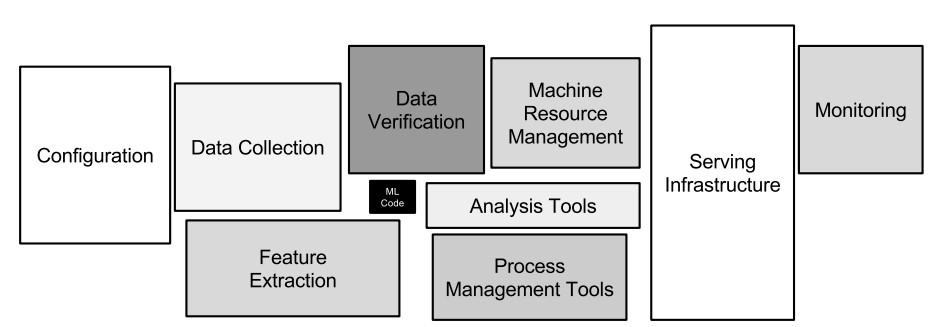
\includegraphics[width=0.8\textwidth]{02-ml-system.png}
  \captionsetup{justification=centering}
  \caption{Gambaran umum komponenen sistem pemelajaran mesin (Sumber:~\cite{NIPS2015_86df7dcf})}\label{fig:ml-system}
\end{figure}

Ternyata, model pemelajaran mesin hanya menjadi sebagian kecil saja dari suatu sistem (\cite{NIPS2015_86df7dcf}).
Bagian yang mendefinisikan model tersebut pada akhirnya hanya menjadi sebagian kecil dari sistem dan merupakan yang paling kecil dibandingkan bagian lainnya (lihat Gambar~\ref{fig:ml-system}).
Hal-hal lain seperti bagaimana melakukan ekstraksi fitur, analisis terhadap data, metode pemberian layanan, dan pengawasan terhadap data menjadi bagian yang lebih besar dalam sebuah sistem pada umumnya.

Oleh karena itu, selain proses pengembangan dan eksperimentasi dari sebuah model, metode sebuah model dapat diberikan lewat layanan juga perlu menjadi hal yang diperhatikan.
Pada praktiknya, pemberian layanan untuk sistem dengan teknologi pemelajaran mesin tidak semudah itu.
Diperlukan perhatian khusus untuk proses pengembangan sistem, khususnya untuk memastikan sistem dapat berjalan dengan mulus.

\subsection{Alur Kerja MLOps}

\begin{figure}[ht]
  \vspace{\baselineskip}
  \centering
  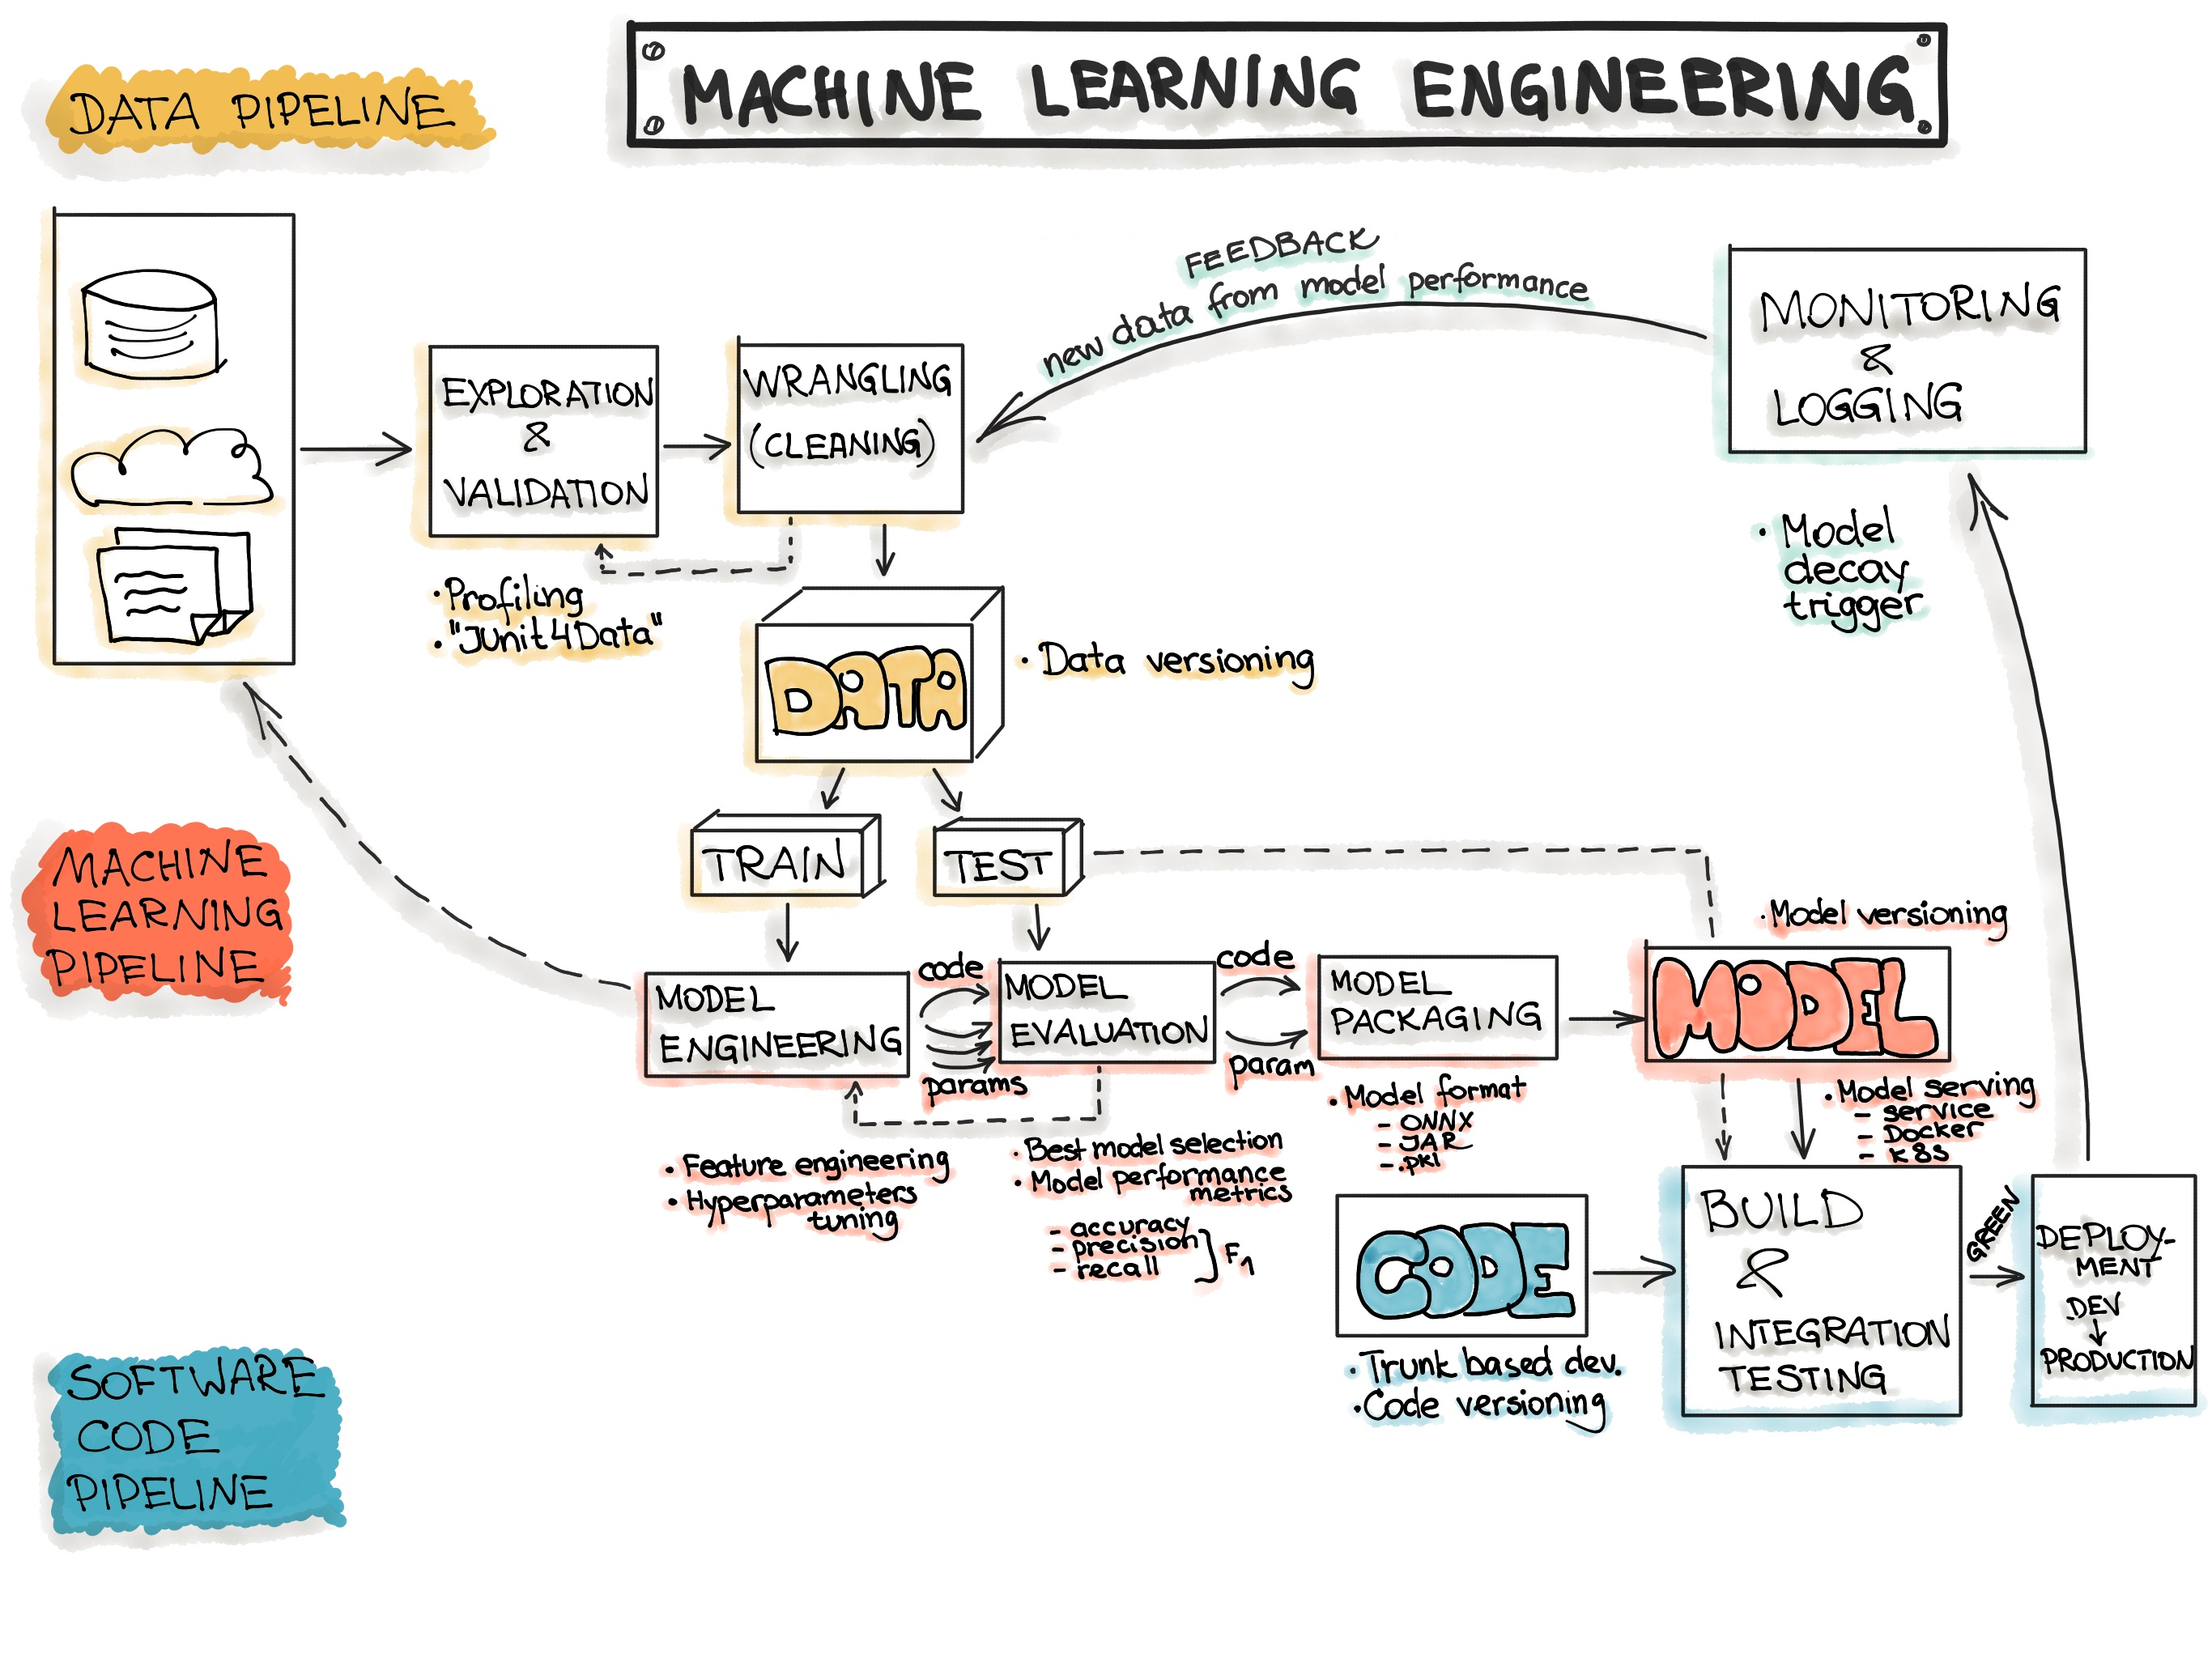
\includegraphics[width=0.8\textwidth]{02-ml-engineering.jpg}
  \captionsetup{justification=centering}
  \caption{Alur kerja umum dalam pembuatan sistem pemelajaran mesin (Sumber:~\cite{mlopsorg})}
\end{figure}

Terdapat tiga tahapan utama dalam alur kerja MLOps (\cite{mlopsorg}).
Alur kerja tersebut adalah sebagai berikut:
\begin{enumerate}
  \item Data Engineering
  \item Model Engineering
  \item Code Engineering
\end{enumerate}

Tugas akhir ini akan membahas secara lebih rinci pada tahap code engineering.
Untuk tahapan lainnya, akan dibahas beberapa hal yang relevan terhadap tahap code engineering.

\subsubsection{Data Engineering}

Tahapan awal dalam bidang ilmu data secara umum seharusnya meliputi pengumpulan data dan persiapan data untuk digunakan dalam analisis.
Secara lebih detailnya, langkah ini dibagi menjadi beberapa tahapan:
\begin{enumerate}
  \item Data Ingestion, yaitu pengumpulan data dari berbagai sumber melalui framework yang ada. 
  \item Data Exploration and Validation, yaitu perlakuan EDA (\textit{Exploratory Data Analysis}) yang meliputi \textit{profiling} terhadap data.
  \item Data Cleaning, yaitu pemrosesan lanjut pada data untuk memperbaiki kesalahan yang ada pada dataset.
  \item Data Labelling, yaitu melakukan labelling kepada dataset yang ada.
  \item Data Splitting, yaitu pemisahan dataset menjadi beberapa bagian yang umumnya adalah untuk \textit{training}, \textit{testing}, dan \textit{validation}.
\end{enumerate}

\subsubsection{Model Engineering}

Setelah melakukan pemrosesan terhadap data, tahapan selanjutnya adalah melakukan pemodelan terhadap dataset yang sudah disiapkan.
Untuk mendapatkan model yang optimal, biasanya tahap ini dibagi menjadi beberapa tahapan yang lebih kecil lagi, yaitu:
\begin{enumerate}
  \item Model Training, yaitu sebuah proses untuk mengaplikasikan algoritma machine learning terhadap training dataset yang ada.
  \item Model Evaluation, yaitu proses evaluasi terhadap model yang dibuat dengan validation dataset atau untuk memastikan apakah model sesuai standar yang diharapkan
  \item Model Testing, yaitu proses \textit{testing} terhadap test dataset atau data yang sengaja disembunyikan untuk menguji kasus-kasus tertentu.
  \item Model Packaging, yaitu proses penyimpanan model yang sudah dibuat dan diuji dalam suatu format file yang dapat digunakan kembali tanpa perlu melakukan pelatihan ulang.
\end{enumerate}

Melalui \textit{framework-framework} pemelajaran mesin seperti Kubeflow, biasanya terdapat fitur untuk melakukan \textit{model versioning}.
Hal ini dilakukan untuk melakukan eksperimen dan pencatatan terhadap \textit{hyperparameter} yang hendak dicoba untuk masing-masing model.
Nantinya, model dengan parameter dan hasil terbaik akan dipilih dan digunakan.

Tahapan ini cukup berpengaruh terhadap tahapan selanjutnya.
Tahapan ini mencakup metode untuk membungkus model atau yang dikenal sebagai \textit{model packaging}.
Bila layanan akan diberikan kepada pihak luar secara masal, biasanya teknologi web akan dipilih untuk melakukan \textit{delivery} bagi layanan tersebut.
Umumnya akan dibuat sebuah API sebagai \textit{interface} agar model dapat dimanfaatkan untuk layanan lain dengan tujuan akhir untuk pelanggan. Detail lengkapnya akan dibahas pada bagian berikutnya. 

\subsubsection{Code Engineering}

Tahapan terakhir dalam MLOps adalah untuk melakukan \textit{code engineering}.
Model yang sudah siap digunakan akan dihubungkan dengan program atau sistem yang ada atau akan ada.
Tahap ini dibagi dalam beberapa tahapan, yaitu:

\begin{enumerate}
  \item Model Serving, yaitu metode agar model yang dibuat dapat di-\textit{deploy} agar dapat diakses pelanggan.
  \item Model Performance Monitoring, yaitu metode untuk melakukan \textit{monitoring} terhadap kinerja model bila diberikan data yang sesungguhnya.
  \item Model Performance Logging, yaitu metode untuk menyimpan \textit{log} dari \textit{request} yang diberikan.
\end{enumerate}

Hal yang menjadi perhatian utama dalam tahap ini adalah metode untuk melakukan \textit{delivery} terhadap model atau yang biasa dikenal sebagai \textit{model serving}.
Banyak pilihan dan \textit{pattern} yang dapat digunakan untuk melakukan \textit{serving}, serta pilihan teknologi yang digunakan untuk \textit{deployment} yang hanya akan dibahas sedikit dalam tugas akhir ini.
\textit{Pattern} untuk melakukan Model Serving akan dibahas pada bagian berikutnya.